\chapter{Monitoring Dashboard Panels}\label{app:panels}

The measurements reported in \cref{chap:results-evaluation} are drawn from the archived k6
summaries and Prometheus snapshots, never from a dashboard image
(\cref{subsec:metrics-pipeline}). The panels collected here serve a different purpose:
they show what the live instrumentation looked like during a run, and they make visible
the shapes over time that a median or a fitted slope necessarily discards.

All five come from the same connector and arm: the Fraunhofer ISST \gls{edc} with its
identity stack enabled. Each panel covers the exact measured window recorded in that run's
provenance file. Only one connector appears, because these panels illustrate the
instrument and do not repeat the comparison.

\begin{figure}[ht]
    \centering
    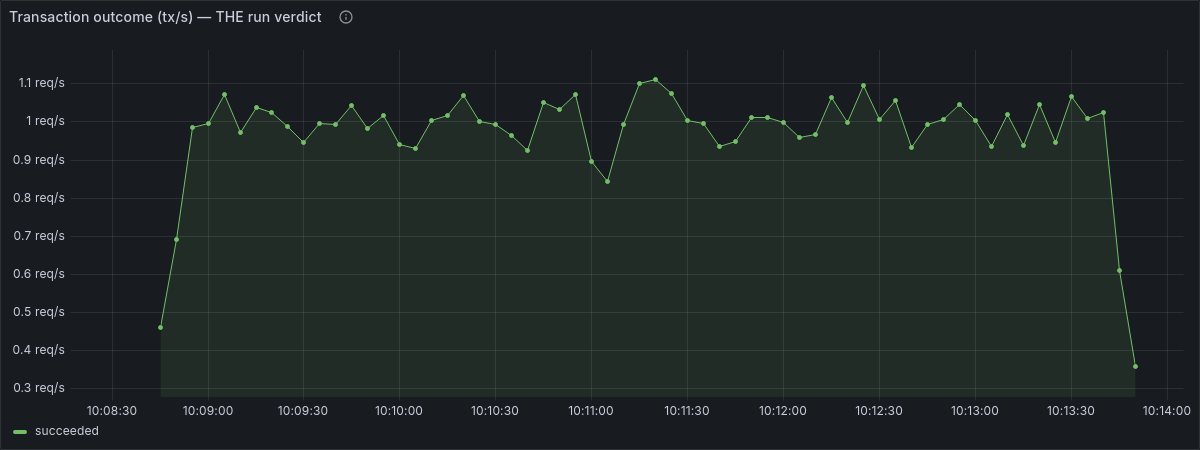
\includegraphics[width=\textwidth]{figures/grafana-rq1-throughput.png}
    \caption[Panel: transaction outcome at the operating point]{Completed transactions per
    second over one measured window at the operating point (\cref{sec:rq1}). The rate
    holds flat for the full five minutes and no failed transactions appear, which is what
    an arm operating below its saturation point looks like.}
    \label{fig:panel-rq1}
\end{figure}

\begin{figure}[ht]
    \centering
    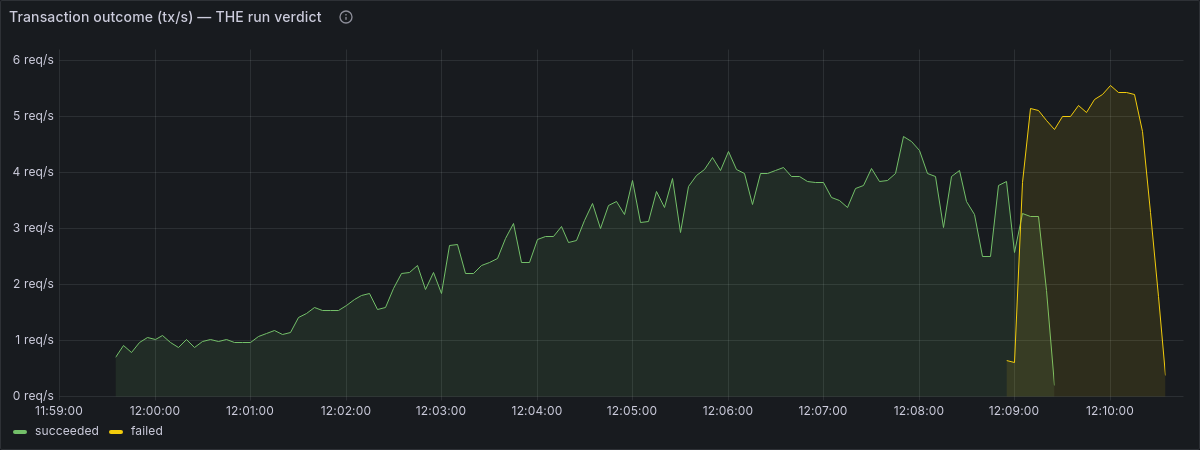
\includegraphics[width=\textwidth]{figures/grafana-rq2-saturation.png}
    \caption[Panel: onset of failure across the load ladder]{Successful and failed
    transactions per second across the load ladder (\cref{sec:rq2}). Successes rise with
    the offered rate to roughly 4.5\,tx/s and then collapse as the failed series takes
    over. \Cref{fig:rq2-saturation} locates the same transition numerically.}
    \label{fig:panel-rq2}
\end{figure}

\begin{figure}[ht]
    \centering
    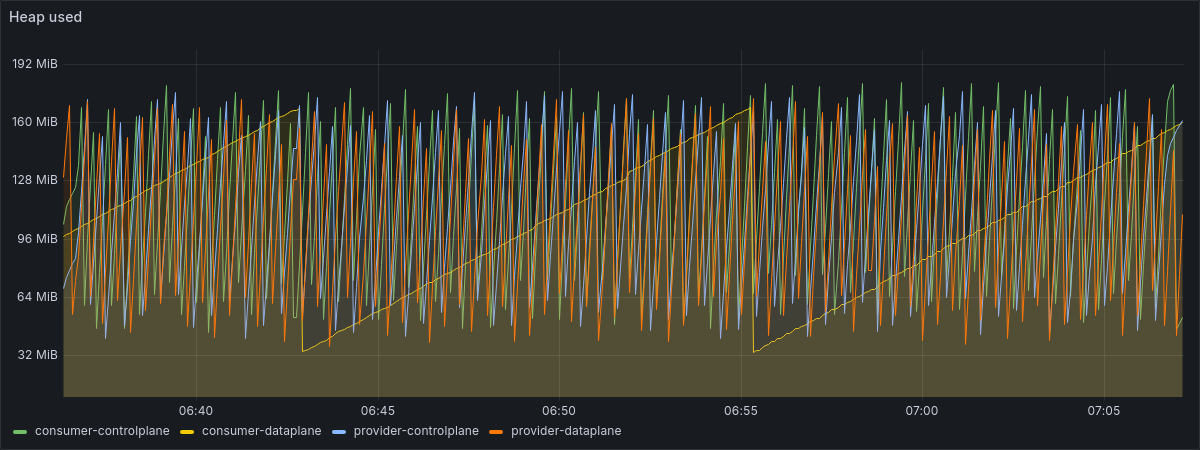
\includegraphics[width=\textwidth]{figures/grafana-rq3-heap.png}
    \caption[Panel: heap occupancy over the endurance run]{\Gls{jvm} heap occupancy per
    runtime over the thirty-minute endurance run (\cref{sec:rq3}). The rapid sawtooth is
    ordinary allocation and collection; the slower climb-and-drop cycle of the consumer
    data plane spans several minutes. Both show why a trend is fitted over every sample
    rather than taken between two of them, and why a thirty-minute window bounds what may
    be concluded about slow growth.}
    \label{fig:panel-rq3}
\end{figure}

\begin{figure}[ht]
    \centering
    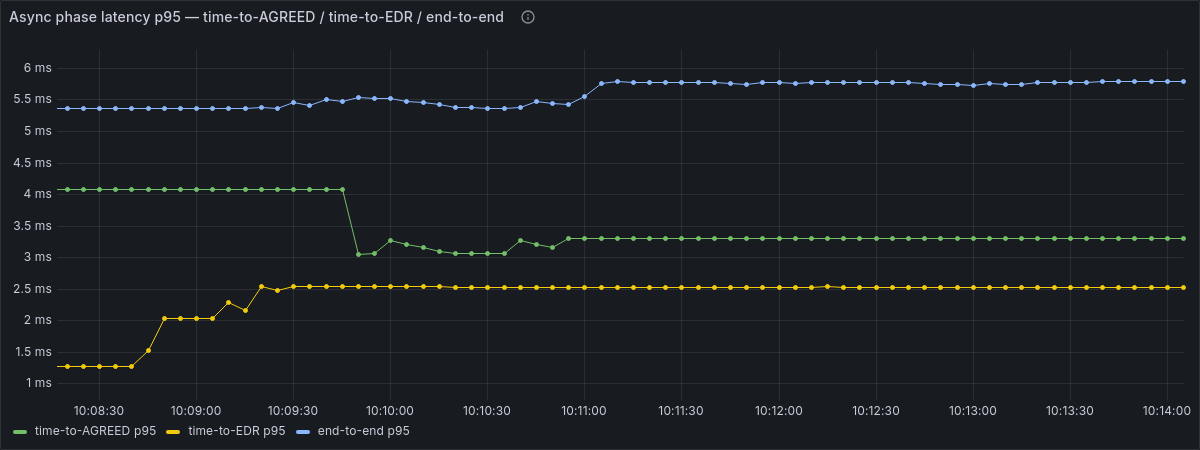
\includegraphics[width=\textwidth]{figures/grafana-rq4-phases.png}
    \caption[Panel: asynchronous phase latency]{Asynchronous phase latency at the
    operating point (\cref{sec:rq4}): time to the agreed contract, time to the endpoint
    reference, and the end-to-end total. The two waits account for almost the whole
    transaction, which is the decomposition \cref{tab:rq4-phases} quantifies.}
    \label{fig:panel-rq4}
\end{figure}

\begin{figure}[ht]
    \centering
    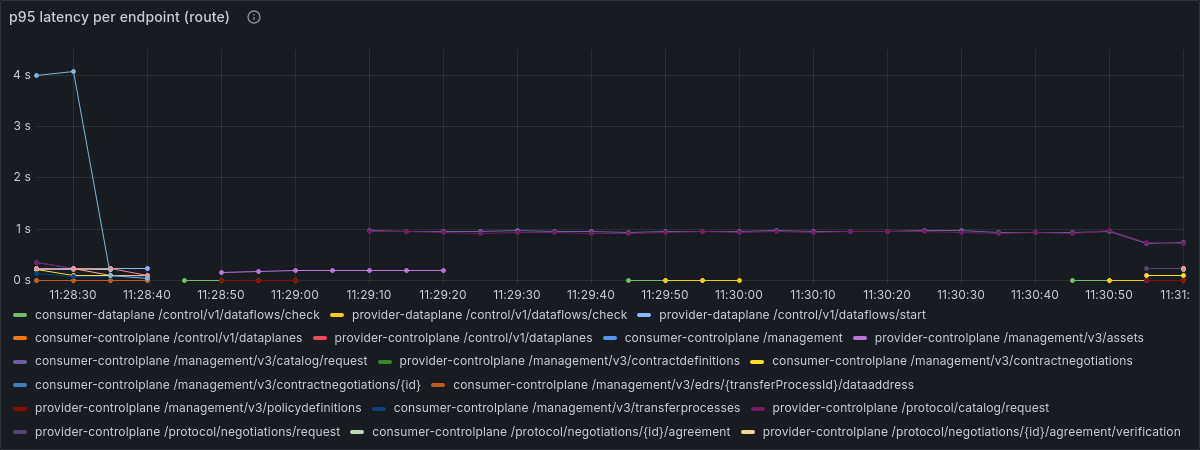
\includegraphics[width=\textwidth]{figures/grafana-rq5-catalog.png}
    \caption[Panel: per-endpoint latency during a catalog sweep]{Server-side
    95th-percentile latency per endpoint during a catalog sweep at 1000 seeded assets
    (\cref{sec:rq5}). Separating the catalog route from the other endpoints is what allows
    catalog cost to be attributed rather than inferred from an aggregate.}
    \label{fig:panel-rq5}
\end{figure}
